\section{The efficiency: definition and loss classes}\label{app:effdef}
\sectionstate{partial}{the old appendices E (definition) and A (loss classes) and the old Table 2, joined; \texttt{rerun/effbudget/single}
(\texttt{radius.py}, \texttt{single\_track*.py}), \texttt{rerun/effbudget/pass1} (\texttt{a1\_recat.py}, \texttt{a1\_table.py});
displays \texttt{papers/paper1\_v2/figs/make\_displays\_v2.py}. v2 2026-11-10: one gallery of all fourteen classes on two pages
replaces fourteen single-event figures (six of which repeated the old gallery).}
\intent{This appendix answers one question: how is the efficiency defined, and where does each lost track go? It
holds the definition and the choice of the matching radius, the variants of the single-track selection, and every loss
class with a real event and the result of trying to recover it.}

\subsection{Definition and matching radius}
\textbf{Denominator.} One reference ray per event: a clean reference track ($\chi^2<1$, four clusters), complete
events only, whose footprint at the chamber lies inside the measured active area. The headline numbers use the whole
active area; \cref{fig:effradius,fig:residuals} are drawn in the interior. Nothing else leaves the denominator: tracks
whose reference may be bent, edge effects, discharges, $\delta$-rays and second particles we cannot separate count as
losses. Only a second particle shown to be independent of the muon (seen in both views with matching charge) leaves
the single-track sample, and then the event is counted with the two-particle events, not dropped
(\cref{sec:twoeff}).

\textbf{Numerator: any candidate.} The reconstruction returns several track candidates per view when the event has
more than one deposit. A muon counts as found when, in each view, the candidate nearest to the reference ray, whatever
rank the reconstruction gave it, is within $R$ of it at the mesh. If the reconstruction keeps the wrong one of two
tracks and the other matches the muon, the event is therefore efficient. Every efficiency quoted for chamber~A uses
this rule (full area: 94.2\,\% of all reference tracks, 94.8\,\% of single tracks; interior: 95.1\,\% and 95.7\,\%). The
stricter kept-track count, in which only the track the reconstruction keeps may match and each view may have at most
two competing strips, gives 91.5\,\% over the full area and 92.3\,\% in the interior; it measures the track selection
as well as the chamber, and is used only to compare chambers (\cref{sec:fleet}). One limit of the any-candidate rule:
the nearest candidates of the two views are chosen independently, so it does not check that they are the same
particle. The pairing of X and Y is studied on its own in \cref{sec:pairing}.

\textbf{The radius.} The efficiency against $R$ (\cref{fig:effradius}) has two regimes: the resolution core, steep up
to about 4\,mm, then a slow rise of 0.1--0.2 points per mm out to 40\,mm. We use $R=5$\,mm, the knee, where the chance
of an accidental match is 0.07\,\%, below the statistical error and 70 times below the inefficiency; $R$ between 4 and
8\,mm moves the efficiency by $-0.5/{+0.7}$ points. The accidental curve is the probability that an unrelated track
lands inside $R$: the chamber's fit of one event is compared with the reference ray of another (event mixing, 20
shifts), scaled by the fraction of events with a fit. It is an upper bound on fakes, since in a real event the muon is
also there.

\begin{figure}[tbp]
  \centering
  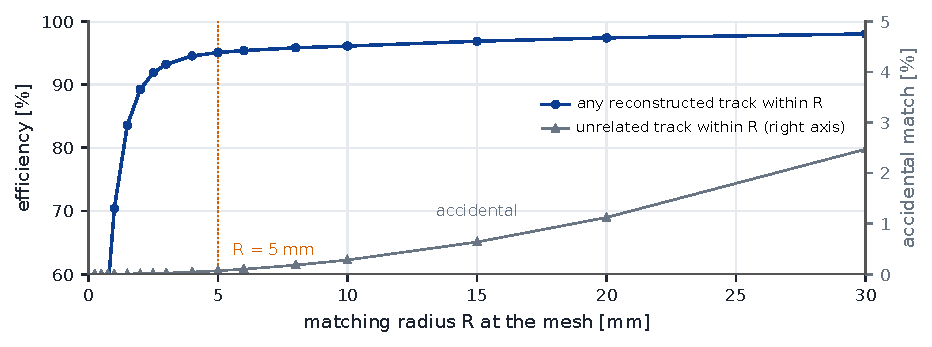
\includegraphics[width=\linewidth]{eff_vs_radius}
  \caption{Efficiency of chamber~A for all reference tracks in the interior (Runs 1 and 2) against the matching radius
  $R$ at the mesh. The muon counts as found if any reconstructed track candidate lies within $R$ of the reference ray
  (95.1\,\% at $R=5$\,mm). Grey, right axis: the probability that an unrelated track (the chamber's fit of another
  event) falls within $R$ of a given reference ray. Dotted: $R=5$\,mm.}
  \label{fig:effradius}
\end{figure}

\textbf{Why 5\,mm and not a few $\sigma$ of the resolution.} The residual at the mesh is not the chamber's
resolution: a Gaussian fit to its core (\crefp{fig:residuals}{a}, $|r|<1.5$\,mm) gives $\sigma=0.55\pm0.02$ (X) and
$0.53\pm0.03$\,mm (Y), of which the chamber contributes about 0.12\,mm (\cref{sec:position}); the rest is the
pointing of the reference ray (0.24 and 0.21\,mm) and the multiple scattering of soft cosmic muons. Its tails are not
Gaussian: only 94 and 92\,\% (X, Y) of the fitted tracks lie within 3$\sigma$ of the reference, 98\,\% within 5\,mm. A
cut at 3$\sigma$ (about 1.6\,mm) would count 11 points of tracks the chamber did find, on the right particle, as
losses, mixing the tails of the reference into the efficiency. The efficiency asks whether the chamber saw the muon;
how well it measured it is the resolution (\cref{sec:tracking}). Between 1.6 and 5\,mm the efficiency rises by 11
points while the accidental rate stays below 0.07\,\%, so those tracks are the muon, measured less well.

\textbf{What lies beyond 5\,mm} (\crefp{fig:residuals}{b}). The grey curve is the distance to another event's
reference ray, scaled as if every fit were unrelated to its muon: an unrelated fit lands mostly more than 40\,mm
away. The data have 7 tracks there against 16\,300 for that hypothesis, so at most about 0.05\,\% of fits are
unrelated, and they contribute less than one of the 244 tracks at 10--20\,mm. The shoulder from 5 to 20\,mm is
therefore correlated with the muon: fits pulled by its $\delta$-rays, a secondary fitted instead of the muon, and
bent reference tracks (the classes below). We cut before it, and count what lies beyond as loss. The residual
distributions are those of the track the reconstruction keeps (both views fitted, no radius cut).

\begin{figure}[tbp]
  \centering
  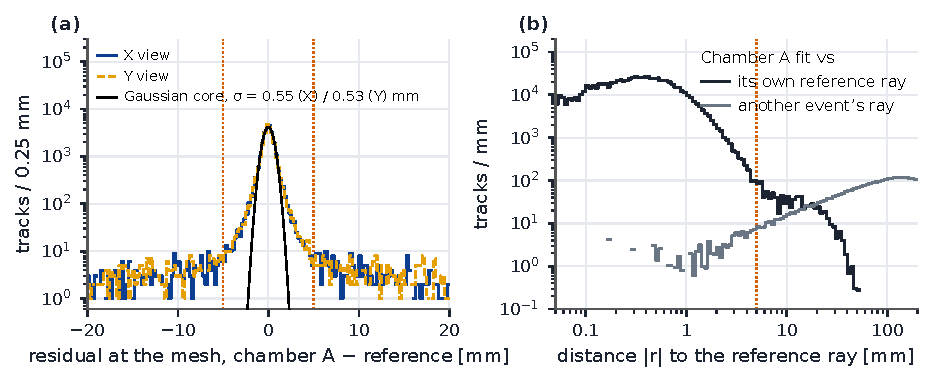
\includegraphics[width=\linewidth]{residuals}
  \caption{The residual distributions of chamber~A behind \cref{fig:effradius}, Runs 1 and 2: (a) per view at the mesh
  (0.25\,mm bins; X solid, Y dashed), (b) radial, with the distance to another event's ray (event mixing, scaled to the
  same number of fits: what the data would be if every fit were unrelated to its muon). Black in (a): a Gaussian fit
  to the core ($|r|<1.5$\,mm), $\sigma=0.55$ (X) and 0.53\,mm (Y). Dotted: $R=5$\,mm. The 5--20\,mm shoulder is
  correlated with the muon, not accidental: the data have 7 tracks beyond 40\,mm where unrelated fits would put
  16\,300.}
  \label{fig:residuals}
\end{figure}

\subsection{Variants of the single-track selection}
\Cref{tab:single} shows how much the single-track efficiency depends on how single tracks are selected. A sample
selected by the chamber's own flag is biased upwards, because a failure that looks like two tracks leaves the sample;
the two-view rule of \cref{sec:single} is not.
\begin{table}[tbp]
  \centering\small
  \caption{Efficiency of chamber~A in the interior, $R=5$\,mm, by selection, Runs 1 and 2. Unlike the numbers of the
  body, this table removes from the denominator the tracks bent between the reference planes and those at the edge of
  the other coordinate (100 tracks), and classifies second particles with an earlier rule; its fourth row therefore
  reads 95.94\,\% where the body has 95.7\,\%.}
  \label{tab:single}
  \begin{tabular}{lr}
    \hline
    selection & efficiency [\%] \\
    \hline
    all tracks & $95.31\pm0.13$ \\
    single, as flagged by the chamber itself (biased) & $97.01\pm0.11$ \\
    single, events with two separate particles removed & $95.30\pm0.13$ \\
    single, all three two-particle configurations removed & $95.94\pm0.12$ \\
    single, $\delta$-ray deposits also removed & $96.75\pm0.11$ \\
    with an independent second particle & $95.9\pm0.8$ \\
    \hline
  \end{tabular}
\end{table}
\askDylan{The bookkeeping agent recommends rebuilding this table on the definitions of the body (94.8/95.7\,\%, nothing
removed), so that the caveat in its caption is not needed. That is a re-run of \texttt{single\_track\_v2.py} with other
settings; not done.}

\subsection{Loss classes}\label{app:losses}
\Cref{tab:losses} follows every reference track in the interior of chamber~A that the kept-track count does not
detect to the one class it ends in, and says whether a change to the reconstruction that does not use the reference
recovers it. The classes count every interior reference track, including those with a second particle, and use the
stricter kept-track count; their fractions are therefore larger than the single-track losses of \cref{sec:single}. One
real event of each class is shown in \cref{fig:gallery1,fig:gallery2}.

\begin{table}[tbp]
  \centering\small
  \caption{Chamber~A interior, 26\,542 reference tracks of Runs 1 and 2 (Run~1: 6\,454), 92.29\,\% detected by the
  kept-track count (Run~1: 92.64\,\%). Every lost track is in exactly one class; the first matching class wins, in the
  order of the table.}
  \label{tab:losses}
  \begin{tabular}{p{5.3cm}rrp{6.6cm}}
    \hline
    class (figure) & \shortstack{Runs 1+2\\{}[\%]} & \shortstack{Run 1\\{}[\%]} & recoverable without the reference? \\
    \hline
% v2: the rows of papers/paper1/sections/a1_table_rows.tex (generated by rerun/effbudget/pass1/a1_table.py) with the
% figure references pointed at the two gallery figures and the wording made public (2026-11-10).
    noise band on a strip patch (\ref{fig:gallery1}a) & 0.22 & 0.22 & largely: band hits are censored (Run 1: 1.43\,\% before that, 0.22\,\% now) \\
    second particle, reference particle fitted, view cut (\ref{fig:gallery1}b) & 1.15 & 1.02 & yes, if a view with two tracks is kept (it is, in the efficiency of \cref{sec:effdef}) \\
    second particle, the other one fitted (\ref{fig:gallery1}c) & 1.51 & 1.47 & no: needs a rule to choose the triggering track \\
    second particle, merged in projection (\ref{fig:gallery1}d) & 0.46 & 0.53 & partly: joint two-track fit with charge corroboration, 25 of the 146 lost tracks of this class get a reference-matched track (Run 1: 3 of 37) \\
    discharge (\ref{fig:gallery1}e) & 0.50 & 0.50 & no \\
    muon + unrelated deposit, over the 50-strip veto (\ref{fig:gallery1}f) & 0.35 & 0.40 & partly: veto off + competing-cluster cut relaxed \\
    shower at the crossing, over the 50-strip veto (\ref{fig:gallery1}g) & 0.81 & 0.67 & no \\
    $\delta$-ray on the track (\ref{fig:gallery2}a) & 0.87 & 0.90 & not with a straight-line model \\
    saturated $\delta$ blob, fit pulled off (\ref{fig:gallery2}b) & 0.93 & 0.84 & no: neither censoring nor a track\,+\,compact-deposit fit (350 saturated views of Run 1: 71\,$\to$\,73\,\% agree) \\
    fit off, no other flag (\ref{fig:gallery2}c) & 0.28 & 0.23 & no \\
    fit failed in one view (formerly the head-on class) (\ref{fig:gallery2}d) & 0.02 & 0.02 & yes: seeding of two-strip clusters (Run 1: 0.26\,\% before, 17 tracks; 0.02\,\% now, none at normal incidence) \\
    position tail, mostly bent reference tracks (\ref{fig:gallery2}e) & 0.17 & 0.20 & no (reference) \\
    edge of the other coordinate (\ref{fig:gallery2}f) & 0.20 & 0.15 & no (geometry) \\
    second deposit, not particle-like (\ref{fig:gallery2}g) & 0.21 & 0.19 & no \\
    other (cuts, charge elsewhere)  & 0.03 & 0.03 & --- \\
    \hline
% ends with the closing \hline
  \end{tabular}
\end{table}

The 7.71\,\% of interior reference tracks that are not detected fall into five groups.

\textbf{The chamber itself: noise bands and discharges (0.72\,\%).} A noise band is a baseline offset over the whole
readout window on a contiguous patch of strips, seen in the X and Y views together. The track itself is clean, but the
view fails the cut on competing clusters. The reconstruction excludes the band from the fit, which brought the class
in Run~1 from 1.43\,\% to 0.22\,\%; under the any-candidate rule of the body half of the remaining band tracks are
found, which is why the body quotes 0.10\,\%. A discharge (0.50\,\%) lights up whole chips, which ring: a real
discharge has 113 strips over threshold, beyond the 50 strips at which the fit is not attempted. It is not
recoverable.

\textbf{A second particle or deposit in the chamber (3.68\,\%).} The largest group. When the chamber sees two
particle-like clusters in a view, three things happen. The reference particle is fitted but the view fails the cut on
competing clusters (1.15\,\%), which the any-candidate rule recovers. The reconstruction fits the other, brighter
particle (1.51\,\%), which needs a rule to choose the triggering track and so cannot be recovered without the
reference. Or the two lie within the 12\,mm in which candidates are merged in one projection, with the fit between
them (0.46\,\%); the joint two-track fit of \cref{sec:twoeff} recovers a reference-matched track in 25 of the 146 lost
tracks of this class. A clean muon with an unrelated deposit elsewhere in the plane can also exceed the 50-strip limit
(0.35\,\%), and a second deposit that is not particle-like (0.21\,\%) is not recovered.

\textbf{$\delta$-rays made by the muon (2.61\,\%).} Three classes, one population of increasing size
(\cref{sec:delta}): a $\delta$-ray along the track (0.87\,\%), a compact saturated one (0.93\,\%), and a shower at the
crossing (0.81\,\%) that exceeds the 50-strip limit. None is recovered.

\textbf{The reconstruction (0.30\,\%).} A fit that is off with no second cluster or saturation flagged (0.28\,\%), and a
fit that failed in one view (0.02\,\%). The latter was a class of tracks at normal incidence whose two-strip cluster in
X was never seeded (0.26\,\% in Run~1); seeding such clusters recovers them.

\textbf{The reference and the geometry (0.37\,\%).} A position tail where the fit agrees with the charge but not with
the reference (0.17\,\%; about two thirds are tracks bent between the reference planes), and tracks at the edge of the
other coordinate (0.20\,\%). These are not losses of the chamber. The remaining 0.03\,\% is not classed further.

\begin{figure}[p]
  \centering
  \figorbox{loss_gallery_1}{loss classes, first seven}
  \caption{The loss classes of \cref{tab:losses}, one real event of chamber~A each (Run~1; both views, strip position
  against drift time, amplitude normalised to the full scale of the ADC; reference track solid black, fit dashed).
  (a) Noise band. (b) Second particle: the reference particle is fitted, but the view fails the cut on competing
  clusters. (c) Second particle: the other one is fitted. (d) Second particle merged with the muon in projection. (e)
  Discharge: whole chips light up and ring. (f) A clean muon and an unrelated deposit, together over 50 strips. (g) A
  shower at the crossing.}
  \label{fig:gallery1}
\end{figure}
\begin{figure}[p]
  \centering
  \figorbox{loss_gallery_2}{loss classes, last seven}
  \caption{The loss classes of \cref{tab:losses}, continued. (a) A $\delta$-ray along the track pulls the fit. (b) A
  saturated $\delta$-ray tilts it. (c) Fit off with nothing flagged. (d) Fit failed in one view: in Y the track lies
  beside a patch of strips with a shifted baseline near the passivated end. (e) Position tail: the fit agrees with the
  charge, the reference does not. (f) Edge of the other coordinate. (g) A second deposit that is not particle-like.}
  \label{fig:gallery2}
\end{figure}
